\label{sub:SpecO}


Our assertions are  %\AssertLang, 
 standard  (\eg properties of the values of expressions,  connectives, quantification \etc)  or  about protection (\ie ${\protectedFrom{{\re}} {{\re}}} $ and 
$ {\inside {{\re}}} $).


% \emph{object capability}. 
% Standard assertions assert properties of the values of fields, implication, quantification etc, as well as ghost fields  which represent user-defined predicates. 
%Object capability assertions express restrictions of  objects' \fbox{eventual authority} on other objects.

\begin{definition}
\label{def:assert:syntax}
%Expressions, $\re$, 
Assertions, $A$,  are defined as follows:

\label{f:chainmail-syntax}
$
\begin{syntax}
%\syntaxElement{\re}{}
%		{
%		\syntaxline
%				{\prg{true}}
%                                {{\alpha}}
%				{{x}}
%                                {\re.f}
%				{\re.f({\overline{\re}})}
%		\endsyntaxline
%		}
%\endSyntaxElement

\syntaxElement{A}{}
		{
		\syntaxline
				{{\re}}
				{{\re} : C}
				{\neg A}
				{A\ \wedge\ A}
				{\all{x:C}{A}}
				{\external{{\re}}}
 				{\protectedFrom{{\re}} {{\re}}} 
				 {\inside {{\re}}} 
		\endsyntaxline
		}
\endSyntaxElement\\
\end{syntax}
$
%In the above, we expect that
\footnote{Addresses in assertions % may contain addresses; 
as \eg  in  $\alpha.blnce > 700$, %. While addresses make little sense in user-written assertions, they are 
are useful when giving semantics to universal quantifiers 
\cf Def. \ref{def:chainmail-semantics}.(\ref{quant1}), {when the local map changes \eg upon call and return, and in general,} for scoped invariants, \cf Def. \ref{def:necessity-semantics}.}

\vspace{.1cm}

{$\fv(A)$ returns the free variables in $A$; for example, $\fv(a\!:\!Account \wedge \forall b:int.[a.\balance = b])$=$\{ a \}$.} 
% {{Moreover, $\fv(A)$ is defined in the obvious way to to return   the free variables in $A$; for example, $\fv(a\!:\!Account \wedge \forall b:int.[a.\balance = b])$=$\{ a \}$.}}

\end{definition}

\forget{
\noindent
\textbf{NOTES}  \notesep % Extended expressions, $\re$, and therefore also 
 Assertions  may contain addresses; \eg   $\alpha.bal > 700$. 
{While addresses make little sense in user-written assertions, they are useful when giving semantics to universal quantifiers 
\cf Def. \ref{def:chainmail-semantics}.(\ref{quant1}), {when the local map changes \eg upon call and return, and in general,} for two-state invariants, \cf Def. \ref{def:necessity-semantics}.(2).}
\notesep The syntax does  not distinguish between fields and ghost fields. For instance, $\prg{a}.\prg{\balance}$ may, in some modules (\eg in \ModA), be a field lookup, while in others (e.g. when the balance is defined though an entry in a lookup table) may involve executing a ghost function. 
% -  $\external {\re}$ is short for $\neg \internal {\re}$. We use these forms freely in the subsequent text without further definition.
% \footnoteSD{{\textbf{NOTE for us} It also allows assertions like $a1.passwd \neq a2.passwd$, whereas in the past we would have written as $\exists x,y.[\ a1.passwd=x \wedge  a2.passwd=y \wedge x\neq y\ ]$.}} \footnoteSD{{TODO compare with oopsla }}
}


\begin{definition}[Shorthands] 
{We write $\internal{\re}$ for $\neg (\external {\re})$}, and
$\extThis$. resp. {$\intThis$} for $\external{\prg{this}}$ resp. $\internal{\prg{this}}$. %, and $\re:\prg{intl}$ as short for $ \neg \external {\re}}$. 
Forms such as $A \rightarrow A'$,  $A \vee A'$, and $\exists x:C.A$  can be encoded.
\end{definition}



\label{def:chainmail-semantics-all}
\label{dup:def:chainmail-semantics}
\noindent
Satisfaction  of Assertions by a module and a state is expressed  through \ $\satisfiesA{M}{\sigma}{{A}}$ \  and defined by cases on the shape of $A$, in definitions \ref{def:chainmail-semantics}  and 
 \ref{def:chainmail-protection}.
 {$M$} is used % might need to 
 to look up the definitions of ghost fields, and to find class definitions to determine whether an object is  external.
 
\footnoteSD{say why we split the def into three defs.} 
\noindent
%\textbf{NOTE}  
%{This is not surprising since the goal of this work is to ensure that external modules cannot break our (internal) module's assertions.}
%\footnoteSD{We need to have clarified internal module earlier.} 
%In most cases, satisfaction depends only on the state $\sigma$, but 
% in some cases it also depends on the module $M$: namely execution of extended expressions   
% -- c.f. Def. \ref{def:chainmail-semantics}, cases (\ref{cExpr}),  (\ref{cInternal}). %,  and (\ref{cExternal}) .

\subsection{Semantics of assertions % \AssertLang 
-- first part}
\label{sect:semantics:assert:standard}

To determine satisfaction of an expression, we    use the evaluation relation, $\eval{M}{\sigma}{e}{v}$,
which says that the expression $e$ evaluates
to value $v$ in the context of state $\sigma$ and module $M$.
%As expressions in \LangOO 
{Ghost fields may be recursively defined, thus evaluation of $\re$ might}
 not  terminate. Nevertheless, the logic of  assertions %$A$ 
 remains classical because recursion is restricted to expressions. %, and not generally to assertions.
\footnoteSD{
The semantics of $\hookrightarrow$ {is} unsurprising 
(see {the appendices %of the full paper 
\cite{necessityFull}).}
We have taken this approach from \citeasnoun{FASE}, which also contains a mechanized Coq proof that assertions are classical \cite{coqFASE}. } %Fig.\ref{f:evaluation}).


\begin{definition}[Satisfaction 
of Assertions -- first part] 
\label{def:chainmail-semantics}
We define satisfaction of an assertion $A$ by a % program 
state $\sigma$ with 
 module $M$ as:
\begin{enumerate}
\item
\label{cExpr}
$\satisfiesA{M}{\sigma}{{\re}}\ \ \ \triangleq \ \ \   \eval{M}{\sigma}{{\re}}{\true}$
\item
\label{cClass}
$\satisfiesA{M}{\sigma}{{{\re}} : C}\ \ \ \triangleq \ \ \   \eval{M}{\sigma}{{\re}}{\alpha}\   \wedge \ \class{\alpha} {\sigma}= C$
\item
$\satisfiesA{M}{\sigma}{\neg A}\ \ \ \triangleq \ \ \   {M},{\sigma}\not\models{A}$
\item
$\satisfiesA{M}{\sigma}{A_1\ \wedge\ A_2}\ \ \ \triangleq \ \ \   \satisfiesA{M}{\sigma}{A_1} \   \wedge \ \satisfiesA{M}{\sigma}{A_2}$
%\item
%$\satisfiesA{M}{\sigma}{A_1\ \vee\ A_2}\ \ \ \triangleq \ \ \   \satisfiesA{M}{\sigma}{A_1}\   \vee \ \satisfiesA{M}{\sigma}{A_2}$
\item
\label{quant1}
$\satisfiesA{M}{\sigma}{\all{x:C}{A}} \ \ \ \triangleq \ \ \   
\forall \alpha.[\   \satisfiesA {M}{\sigma} {\alpha:C}  \ \Longrightarrow   \ \satisfiesA{M}{\sigma} {A[\alpha/x]} \ ] $

%\item
%\label{quant2}
%$\satisfiesA{M}{\sigma}{\ex{x:C}{A}}$ \ \ \ iff \ \ \  
% {$\exists \alpha.[\ \GRelevant \alpha \sigma \wedge  \satisfiesA {M}{\sigma} {\alpha:C}  \ \wedge \ \satisfiesA{M}{\sigma} {A[x/\alpha]}\ ]$.} 
%\item
%\label{cInternal}
%$\satisfiesA{M}{\sigma}{\internal{{\re}}}$ \ \ \ iff \ \ \   $\satisfiesA{M}{\sigma}{{{\re}} : C} \ \wedge\ \ C \in M$
\item
\label{cExternal}
$\satisfiesA{M}{\sigma}{\external{{\re}}} \ \ \ \triangleq \ \ \  \exists C.[\ \satisfiesA{M}{\sigma}{{{\re}} : C} \ \wedge \ C \notin M \ ]$
\end{enumerate}
\end{definition}

 
Note that while execution takes place in the context of one or more modules, $\Mtwo$, satisfaction of assertions considers \emph{exactly one} module  $M$ -- the internal module. 
{$M$} is used  to look up the definitions of ghost fields, and to % find class definitions to 
 determine whether objects are  external.

\subsection{Semantics of Assertions - second part}  

\label{sect:protect}
% Long motivation.
% However the motivation from sect 2 shoud be sufficient
%In the object capabilities model \cite{MillerPhD}, \emph{access} to a capability (called a \emph{permission} in \cite{MillerPhD}
% is a necessary precondition  for producing a given effect;  as expressed by the principle that ``authority (to cause an effect) implies eventual permission'' \cite{permissionAuthority}.
%As   in \S \ref{sec:shop}, and also \cite{OOPSLA22}, if no external object has eventual access for a given capability, then the corresponding effect cannot occur.
% Specifically,  we say that $o$ \emph{has eventual access to} $o'$, to mean  that $o$ either currently has or will acquire direct access to $o'$ in the future \cite{permissionAuthority}.
%
%
%
%Given this, it becomes essential to determine whether eventual access exists in a given state. 
%Unfortunately, this determination is undecidable, as it depends not only on the current object graph but also on the program code being executed.
%
%In this work, we over-approximate lack of eventual access through a combination of two properties: one pertaining to the state, and the other to the internal code. 
%The  property pertaining to the state is $\satisfiesA{M}{\sigma} {\inside {\alpha}}$, \ie that   $\alpha$ is \emph{protected},
%\ie that   {no locally reachable external objects have direct access to $o$.}
%% on any path from a locally reachable object to $o$, the penultimate object  is internal. 
%The  property pertaining to the program is that it preserves the protection of   $o$.
%%
%We can see that if $o$ is protected and the internal code preserves its protection, then no external object can gain eventual access to $o$.

In \S \ref{sect:approach:protection} we % discussed the importance of a guarantee that there will be no external access to a capability, and how this can be modelled 
introduced protection -- we will now formalize this concept. % in Def. \ref{def:chainmail-protection-from}.

 An object is protected from another object, $\protectedFrom{{\alpha}} {{\alpha_{o}}}$, if 
the two objects are not equal, and no external object reachable from $a_o$ has a field pointing to  $\alpha$.
This ensures that the last element on any path leading from $\alpha_o$ to $\alpha$
in an internal object.   
 

An object is protected,  $\inside{{\alpha}}$,  if no external object
reachable from any of the current frame's arguments has a field
pointing to $\alpha$; and furthermore, if the receiver is external,
then
no parameter to the current method call directly refers to $\alpha$.
%
This  ensures that no external object reachable from the current
receiver or arguments can ``obtain'' $\alpha$, where obtain $\alpha$ is either direct access through a field,  
 or by virtue of the method's receiver %having access to
 being able to see all the arguments.
 


 
\begin{definition}[Satisfaction 
of Assertions  -- Protection] 
\label{def:chainmail-protection-from}
\label{sect:semantics:assert:prtFrom}
 \label{def:chainmail-protection}
-- continuing definitions in \ref{def:chainmail-semantics}:
\begin{enumerate}
\item
\label{cProtected}
 $\satisfiesA{M}{\sigma}{\protectedFrom{{\alpha}} {{\alpha_{o}}}}   \ \ \ \triangleq $ 
  \begin{enumerate}
 \item
$\alpha\neq \alpha_0$,
 % \ \ \ \  and 
 \item
$\forall \alpha'.\forall f.[\ \alpha' \in {\Relevant {\alpha_o} {\sigma}} \wedge\   \satisfiesA{M}{\sigma}{\external {\alpha'}} 
\ \ \Longrightarrow \ \  
  \interpret {\sigma} {\alpha'.f} \neq \alpha     \ ] $.
\end{enumerate}
\item
\label{sect:semantics:assert:prt}
$\satisfiesA{M}{\sigma} {\inside {\alpha}}  \ \ \ \triangleq \ \ \   $
 \begin{enumerate}
\item
 $\satisfiesA{M}{\sigma}{\extThis}\ \ \Longrightarrow\ \ \forall x\!\in\! \sigma.\ \satisfiesA{M}{\sigma}{x\neq \alpha}$,
 \item
$\forall \alpha'.\forall f.[\ \alpha' \in {\LRelevantO {\sigma}} \wedge\   \satisfiesA{M}{\sigma}{\external {\alpha'}} 
\ \ \Longrightarrow \ \  
  \interpret {\sigma} {\alpha'.f} \neq \alpha     \ ] $.
  \end{enumerate}
\end{enumerate}
Moreover,  \\
$\strut \ \ \ \ \ \  (3) \ \  \satisfiesA{M}{\sigma}{\protectedFrom{{\re}} {{\re_{o}}}}$ $ \triangleq$
$\exists \alpha, \alpha_{o}. [\  \eval{M}{\sigma}{{\re}}{\alpha}\ \wedge\ \eval{M}{\sigma}{{\re_0}}{\alpha_0} \  \wedge \ 
  \satisfiesA{M}{\sigma}{\protectedFrom{{\alpha}} {{\alpha_{o}}}}\   ]$, \\
  $\strut \ \ \ \ \ \ (4) \ \ \satisfiesA{M}{\sigma}{\inside{\re}}$  $\triangleq$
 $\exists \alpha. [\   \eval{M}{\sigma}{{\re}}{\alpha}\ \wedge \   \satisfiesA{M}{\sigma}{\inside{\alpha}} \  ]$. 

 \end{definition} 
 
 We illustrate ``protected'' and ``protected from'' in Fig.  \ref{fig:ProtectedBoth} in \S \ref{s:outline}.
% that appendex commented out from all version of main.tex
   and    Fig.  \ref{fig:ProtectedFrom} in App. \ref{appendix:assertions}.
%
In general,  $\protectedFrom{{\alpha}} {{\alpha_{o}}}$ ensures that $\alpha_o$ will get access to $\alpha$ only if another object 
 % an internal object 
 grants that access.
Similarly, $\inside \alpha$ ensures that during execution of the current method, no external object will get direct access to $\alpha$ unless some internal object grants that access\footnote{This is in line with the motto "only connectivity begets connectivity" from \cite{MillerPhD}.}.
Thus, protection together with protection preservation  (\ie no internal object gives access) guarantee
%are sufficient but not necessary conditions for 
lack of eventual external access.  

 
\footnoteSD{JAMES' comment: If is possible that ``we'' do not know the complete heap (eg we only know about the green stuff.) how do we know whether an object is protected. The answer is that we do not know that it is protected, but we do know that our code guarnartees poreservation of protectedness.
}  
 
 \subsubsection*{Discussion} 
Lack of  eventual 
direct access is a central concept in the verification of code with calls to and callbacks  from untrusted code.
% ARGHHH a joke citatiion? \cite{praiseYou}.   
%Unmediated access is essentially \citet{MillerPhD}'s permission: that we have a ``first
%class'' reference to the capability; that we can call any 
%method in the capability's public interface; that we can
%store or save or present the capability to any other
%object to which we've been introduced
%%\footnote{``nobody can ever be introduced in a ball-room''}
It has already been over-approximated in several different ways, \eg
2nd-class \cite{rompf-second-class-oopsla2016,rompf-dont-pop-second-class-ecoop2022}
or borrowed (``2nd-hand'') references
\cite{boyland-promises-icse1998,boyland-aliasburying-spe2001},
 textual modules \cite{OOPSLA22},
information flow \cite{ddd}, runtime
checks \cite{secure-io-fstar-popl2024},
abstract data type exports \cite{vmsl-pldi2023},
  separation-based invariants 
Iris \cite{iris-wasm-pldi2023,cerise-jacm2024},
-- more in  \S~\ref{sect:related}.
In general, protection is applicable in more situations (i.e.\ is less
restrictive) than most of these approaches,
 although more restrictive than the ideal ``lack of eventual access''. 
\footnoteSD{ HER WHAT IT USED TO SAY: the contrapositive ideal that lack of eventual access ensures
lack of effect. Note that ``cannot get direct access'' does not generally imply ``is protected''. 
}





\noindent
\begin{flushleft}
\begin{tabular}{@{}lr@{}}
  \begin{minipage}{.85\textwidth}
   {An alternative definition might consider $\alpha$ as protected from $\alpha_o$, 
if   any path from $\alpha_o$ to $\alpha$ goes through at least one internal object.
With this definition, $o_4$ would be protected from $o_1$ in the heap shown here.
However,  $o_1$ can make a call to $o_2$, and  this call could  return $o_3$. 
Once $o_1$ has direct access to $o_3$, it can also get direct access to $o_4$. 
The example justifies our current definition.  
}
\end{minipage}
& 
\begin{minipage}{.18\textwidth}
\resizebox{2cm}{!}{
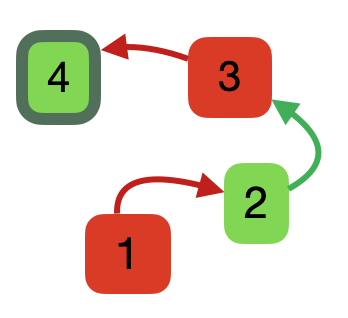
\includegraphics[width=\linewidth]{diagrams/altDef.png}
} 
\end{minipage}
\end{tabular}
\end{flushleft}


%Protection --- \sdN{objects to which external objects may not get %which objects can get 
%unmediated access} % to which other objects 
%---  is  a crucial concept: It enables
%the verification code in the open world, % even in the presence of
%with calls to and callbacks 
%from untrusted code.
%% ARGHHH a joke citatiion? \cite{praiseYou}.   
%Unmediated access is essentially \citet{MillerPhD}'s permission: that we have a ``first
%class'' reference to the capability; that we can call any 
%method in the capability's public interface; that we can
%store or save or present the capability to any other
%object to which we've been introduced
%%\footnote{``nobody can ever be introduced in a ball-room''}
%(compare
%2nd-class \cite{rompf-second-class-oopsla2016,rompf-dont-pop-second-class-ecoop2022}
%or borrowed (``2nd-hand'') references
%\cite{boyland-promises-icse1998,boyland-aliasburying-spe2001}
%which are restricted in some way),
%without reference to some owning class or defining module.
%We discuss alternative designs,
%ranging from overly simplistic textual modules \cite{OOPSLA22},
%information flow \cite{ddd}, runtime
%checks \cite{secure-io-fstar-popl2024},
%abstract data type exports \cite{vmsl-pldi2023},
%to automated separation-based invariants in
%Iris \cite{iris-wasm-pldi2023,cerise-jacm2024},
%in section~\ref{sect:related}.
%In general, protection is applicable in more situations (i.e.\ is less
%restrictive) than most of these approaches,
% \sdN{although more restrictive than the ideal "lack of eventual permission"}. 
%\footnoteSD{ HER WHAT IT USED TO SAY:
%the contrapositive ideal that lack of eventual permission ensures
%lack of effect. Note that ``cannot get direct access'' does not generally imply ``is
%protected''


 
